\documentclass{article}
%\usepackage[a4paper, total={6in, 8in}]{geometry}
\usepackage{geometry}
 \geometry{
 a4paper,
 total={210mm,297mm},
 left=20mm,
 right=20mm,
 top=-2mm,
 bottom=2mm,
 }
%\usepackage[margin=0.5in]{geometry}

\usepackage{amsmath,amssymb,amsfonts}
\usepackage{ifpdf}
\usepackage{float}
\usepackage{cite}
\usepackage{algorithmic}
\usepackage{array}
\usepackage{mdwmath}
\usepackage{pdfpages}
\usepackage{mdwtab}
\usepackage{eqparbox}
\usepackage{cite}
\usepackage{multirow}
%\onecolumn
%\input{psfig}
\usepackage{color}
\usepackage{multicol}
\usepackage{textcomp}
\usepackage{comment}
\usepackage{xcolor}
\usepackage{hyperref}
\usepackage{graphicx}
\usepackage{listings}
\usepackage[ruled,vlined]{algorithm2e}
\usepackage{hyperref}
\hypersetup{
    colorlinks=true,
    linkcolor=olive,
    filecolor=magenta,      
    urlcolor=blue
}
\setlength{\textheight}{23.5cm} \setlength{\topmargin}{-1.05cm}
\setlength{\textwidth}{6.5in} \setlength{\oddsidemargin}{-0.5cm}
\setlength{\parskip}{1em}
\renewcommand{\baselinestretch}{1}
\pagenumbering{arabic}
\usepackage{ragged2e}
\renewcommand{\baselinestretch}{1.5}

\begin{document}

\textbf{
\begin{center}
{
\large{School of Engineering and Applied Science (SEAS), Ahmedabad University}\vspace{4mm}
}
\end{center}
%
\begin{center}
\large{B.Tech(CSE) Semester IV: Probability and Stochastic Processes (MAT 277) }\\ \vspace{3mm}
\end{center}
}
\begin{itemize}
\item Group No: BB15
\item Names (Roll No.s): \begin{itemize}
    \item Kirtan Kalaria (AUL2020005)
    \item Jay Patel (AU1920156)
    \item Christian Noel Wajiri (AU1920174)
    \item Dinesh Nariani (AU1920128)
    \item Smit Shah (AU1920088)
    \item Luv Ghodasara (AU1920173)
    \item Tanmay Srivastava (AU1920084)
    \end{itemize}\end{itemize}
    \BlankLine \BlankLine
\begin{center}
\textbf{{Project Title: How many genes are involved in schizophrenia? A simple simulation}} \end{center}

\section {Justify how probabilistic model/PSP concept is used in your project. How is uncertainty modeled?}

\subsection{Modeling of physical/real-time uncertain Problem, Study of any existing probability based models, etc.}
  
Our first objective was to tap into the concepts explained and the underlying mathematics of the research paper. We sought to understand it and reproduce some of the results. The paper starts with acknowledging the success of polygenic threshold models to model the risk of schizophrenia morbidity in relatives of patients. (Early on, we recognized that since offsprings are relatives, also through the succeeding generations.) Such models attribute the risk to a combined effect of a large number of genes, where each gene contributes sparingly. Independent effect of any single gene on the risk is negligible. Hence, in order to obtain statistically stable results, the sample size required will be very high, which may or may not be practical.
  
The authors of the paper aim to address the following two questions:
\begin{itemize}
    \item How many genes are involved in schizophrenia?
    \item How large a sample is required for stable detection of a true genetic difference?
\end{itemize}

They used a primitive probabilistic model with sufficient simplicity for ease of calculations, but at the same time, relevant enough to actually represent the situation. The assumptions can be referred from the paper itself. Here on, we proceed assuming the reader has full knowledge of the terminology and assumptions.

By the polygenic approach and making some assumptions,the number of pathogenic genes (genetic load) in the General Population (here forth GP) follows a binomial distribution $B(N, p_{G\_GP})$, where for each integer k, such that $0\leq k\leq N$, the y-value can be observed as the probability (of genetic load of k in any random person in GP) as well the frequency (of genetic load in a person being exactly k in the GP), which is not surprising as it is merely the fundamental idea of statistics. $p_{G\_GP}$ here is the probability that an individual from the GP has a pathogenic genotype (homozygous: AA or heterozygous: Aa). For the genetic load of k, the frequency is:

\begin{center}
$p_{\_GP}(k) = ^nC_{k} \cdot (p_{G\_GP})^k \cdot\ ( 1-p_{G\_GP})^{n-k}$
\end{center}

In the distribution, all cases where the genetic load k is greater than or equal to $N\cdot T$, usually in the tail region, represent the sub-population that have the proper genetic conditions be schizophrenic, which is the patient population(here forth PP). However, only a ratio of those people, defined as penetrance, actually develop the illness and are patients. Looking at it the other way, everyone in PP has the probability of being a patient equal to penetrance. Hence, the sum of frequencies for PP multiplied by the penetrance, gives us the prevalence. This is represented by the equation:
  
\begin{center}
$prevalence = penetrance \cdot \sum_{k=NT}^{N} (p_{GP}(k))$
\end{center}
  
The aim is to segregate the patient population(here forth PP) from the above binomial distribution for genetic load in GP, using known ground truth value of prevalence ($2.24\%$) and a reasonably selected constant value of penetrance (0.5) based on known information.
  
Initially, the value of $p_{G\_GP}$ is unknown. However, the authors mention that one should try different values and pick the one that results in the resulting prevalence to match the known value. In the following figure for $B(N, p_{G\_GP})$, they hint at an iterative process of starting with a low value and gradually increasing it until the target prevalence value is achieved.
  
\begin{figure}[htbp]
    \centering
    \includegraphics[scale=0.3]{Images/Binomial of GP.jpg}
    \caption{Incrementing $p_{G\_GP}$ such that the area of the binomial PMF for $k\geq N\cdot T$} is $2.24\%$
    \label{fig:my_label}
\end{figure}
  
Since the all genotype and allele frequencies in the general population are in Hardy Weinberg Equilibrium (hence forth HWE), we can express them as follows:
  
\begin{center}
If $Pr(A) = p_{A\_GP} = q$ and $Pr(a) = p$, then
\end{center} \begin{center}
$p + q = 1 \Longrightarrow Pr(a)=1-p_{A\_GP}$ and
\end{center} \begin{center}
$Pr(AA) = q^2 = (p_{A\_GP})^2$, $Pr(Aa) = 2(1-p_{A\_GP})(p_{A\_GP})$, and $Pr(aa)=p^2=(1-p_{A\_GP})^2$
\end{center} \begin{center}
Finally, $p_{G\_GP} =Pr(AA)+Pr(Aa) = 1 - Pr(aa) =  1-(1-p_{A\_GP})^2$
\end{center}
  
It is apparent from that above equation how the pathogenic allele frequency in GP, $p_{A\_GP}$ can calculated using the $p_{G\_GP}$.
  
The frequencies of the two alleles at any locus are in HWE in the GP but not necessarily in the PP, as they do not are not an isolated sub-population. It can only be assumed PP is in HWE if they mate only among their own population, which in turn is neither assumed nor the general case. The same applies for the non-patient population(here forth NP). Although the frequency of pathogenic allele is higher in the PP than in the GP, the ratio of homozygote alleles to heterozygote alleles in the PP and the GP are the same, because PP is a subset of the GP.
  
Then the mean genetic load and the pathogenic genotype and allele frequencies in the PP: $p_{G\_PP}$ and $p_{A\_PP}$ are calculated as
  
$$Mean\_load_{PP}=\frac{\sum_{k=NT}^{N} (p_{GP}(k)\cdot k)}{prevelance/penetrance}=\frac{\sum_{k=NT}^{N} (p_{GP}(k)\cdot k)}{\sum_{k=NT}^{N} p_{GP}(k))}$$
$$ p_{G\_PP} = \frac{Mean\_load_{PP}}{N}$$
  
$$p_{A\_PP} = \frac {p_{G\_PP} \cdot p_{A\_GP}}{p_{G\_GP}}$$
  
After that, the pathogenic allele frequency in the NP($p_{A\_NP}$) can be calculated from the very straightforward and intuitive equation:
  
$$p_{A\_GP}=  p_{A\_PP} \cdot prevalence +p_{A\_NP} \cdot (1- prevalence)$$
  
Using the fact that the the ratio of homozygote alleles to heterozygote alleles in the NP is the same as that in GP (and PP) because NP is also a subset of GP, we calculate the pathogenic genotype frequency for NP sub-population as:
  
$$p_{G\_NP} = \frac {p_{A\_NP} \cdot p_{G\_GP}}{p_{A\_GP}}$$
  
\subsection{Include Block/State diagram (Optional)}
%\item Explain the probabilistic model used to solve the problem
Not required; it is easily understood by reading 1.1 and the code.

\section{Clearly enlist the new things done in the coding part, excluding the shared code. [If no new code is written/added/modified, then please write NA]}
The shared code was wrong in many ways. Firstly, the graphs were hard-coded. Secondly, the implementation of the mathematics was incorrect. Lastly, the code was very unorganized. So we decided to drop it and start anew.
\begin{enumerate}
    \item
    First, we set up functions to calculate the pathogenic genotype and allele frequencies in all populations.
    \item
    Then, we reproduce figures 2 and 3 of the research paper.
    \item
    After that, we set up functions to calculate the pathogenic frequencies and prevalence in offsprings, which will pave the way for the innovation component.
    \item
    Then, we simulate PP inbreeding and define a function to plot pathogenic frequency in GP and PP and the prevalence (always in GP).
    \item
    Out of curiosity, we try to regenerate figure 5 of the research paper as well but that is still work in progress and is beyond the requirements of this project.
\end{enumerate}

\section{Contribution of team members}	
\subsection{Technical contribution of all team members }
\begin{table}[h]
\centering
\label{tab:my-table}
\begin{tabular}{|l|c|c|c|c|c|c|c|}
\hline
Tasks                & Kirtan K.             & Jay P.                & Dinesh N.             & Christian N. W.       & Smit S.               & Tanmay S. & Luv P. \\ \hline
Planning the project & \checkmark & \checkmark &    \checkmark                   & \checkmark & \checkmark & -         & -      \\ \hline
Coding               & \checkmark & \checkmark & \checkmark & -                     & -                     & -         & -      \\ \hline
Innovation           & \checkmark & -                     & -                     & -                     & -                     & -         & -      \\ \hline
\end{tabular}
\end{table}
\subsection{Non-Technical contribution of all team members}
    \begin{table}[h]
    \centering
    \label{tab:my-table}
    \begin{tabular}{|l|c|c|c|c|c|c|c|}
    \hline
    Tasks                  & Kirtan K.                 & Jay P.                    & Dinesh N.                 & Christian N. W.           & Smit S.                   & Tanmay S.                 & Luv P.                    \\ \hline
    Concept map            & \checkmark & \checkmark & \checkmark & \checkmark & \checkmark & \checkmark & \checkmark \\ \hline
    Understanding article  & \checkmark & \checkmark & -                         & \checkmark & \checkmark & -                         & -                         \\ \hline
    Exploration of results & \checkmark & -                         & \checkmark & \checkmark & \checkmark & -                         & -                         \\ \hline
    \end{tabular}
    \end{table}
  
\section{Any innovation done considering the society/neighborhood problem?}

The authors assessed the risk of schizophrenia morbidity in the relatives of patients using combinations and statistical manipulation of the risk in the three populations. Then we realized that since offsprings are also relatives, risk assessment of the offsprings is equivalent to that of the defined crossing (PP×PP, PP×NP and NP×NP) subset of the successive generation.
  
For PP×PP, PP×NP and NP×NP offsprings, the genotype frequency can be calculated from the allele frequencies in the parental germ cells. The authors so not mention the underlying mathematics in the appendix, however, it was not very difficult to derive.
  
Now, assume that the parents are called parent 1 and parent 2. For a particular gene at a particular locus, the parents will pass down their alleles from their own genes. Let the alleles be $X_1,\,X_2,\, X_3,\,\textit{and }X_4$. Consider the following Punnett Square.

\begin{table}[h]
\centering
\label{tab:my-table}
\begin{tabular}{llll}
                                               &                            & \multicolumn{2}{c}{Parent 1}                                   \\ \cline{3-4} 
                                               & \multicolumn{1}{l|}{}      & \multicolumn{1}{l|}{$X_1$}        & \multicolumn{1}{l|}{$X_2$} \\ \cline{2-4} 
\multicolumn{1}{c|}{\multirow{2}{*}{Parent 2}} & \multicolumn{1}{l|}{$X_3$} & \multicolumn{1}{l|}{$X_{1}X_{3}$} & \multicolumn{1}{l|}{$X_{2}X_{3}$}    \\ \cline{2-4} 
\multicolumn{1}{c|}{}                          & \multicolumn{1}{l|}{$X_4$} & \multicolumn{1}{l|}{$X_{1}X_{4}$}           & \multicolumn{1}{l|}{$X_{2}X_{4}$}    \\ \cline{2-4} 
\end{tabular}
\end{table}

Then,

\begin{equation}
\begin{split}
&Pr(\textit{Offspring has pathogenic genotype})
\\&=\sum{(i,j)=(1,3),(1,4),(2,3),(2,4)} Pr(\textit{Offspring genotype is }X_iX_j)\times Pr(X_iX_j\textit{ is p.g.})
\\&=\sum_{(i,j)=(1,3),(1,4),(2,3),(2,4)} \frac{1}{4}\times Pr(X_iX_j\textit{ is p.g.})
\\&=\sum_{(i,j)=(1,3),(1,4),(2,3),(2,4)} \frac{1}{4}\times Pr(X_iX_j\textit{ is AA or Aa})
\\&=\frac{1}{4}\sum_{(i,j)=(1,3),(1,4),(2,3),(2,4)} Pr(X_iX_j\textit{ is AA or Aa})
\\&=\frac{1}{4}\sum_{(i,j)=(1,3),(1,4),(2,3),(2,4)} Pr(X_iX_j\textit{ is AA})+Pr(X_iX_j\textit{ is Aa})
\\&=\frac{1}{4}\sum_{(i,j)=(1,3),(1,4),(2,3),(2,4)} [Pr(X_i=A)\cdot Pr(X_j=A)]+[Pr(X_i=A)\cdot Pr(X_j=a)]+[Pr(X_i=a)\cdot Pr(X_j=A)]
\\&=\frac{1}{4}\sum_{(i,j)=(1,3),(1,4),(2,3),(2,4)} Pr(X_i=A)[Pr(X_j=A)+Pr(X_j=a)]+[Pr(X_i=a)\cdot Pr(X_j=A)]
\\&=\frac{1}{4}\sum_{(i,j)=(1,3),(1,4),(2,3),(2,4)} Pr(X_i=A)+[Pr(X_i=a)\cdot Pr(X_j=A)]
\\&=\frac{1}{4}\sum_{i=1,2} \left \{  Pr(X_i=A)+[Pr(X_i=a)\cdot Pr(X_3=A)]\right \} + \left \{  Pr(X_i=A)+[Pr(X_i=a)\cdot Pr(X_4=A)]\right \}
\\&=\frac{1}{4}\sum_{i=1,2} 2Pr(X_i=A) + Pr(X_i=a)[Pr(X_3=A)+Pr(X_4=A)]
\\&=\frac{1}{4} \left \{2Pr(X_1=A)+2Pr(X_2=A) + [Pr(X_1=a)+Pr(X_2=a)][Pr(X_3=A)+Pr(X_4=A)] \right \}
\\&=\frac{1}{4} \left \{2Pr(X_1=A)+2Pr(X_2=A) + [1-Pr(X_1=A)+1-Pr(X_2=A)][Pr(X_3=A)+Pr(X_4=A)] \right \}
\\&=\frac{1}{4} \{2Pr(X_1=A)+2Pr(X_2=A)+2Pr(X_3=A)+2Pr(X_4=A)
\\&\hspace{6cm}-[Pr(X_1=A)+Pr(X_2=A)][Pr(X_3=A)+Pr(X_4=A)]\}
\\&=\frac{1}{4} \left \{2p_{A\_ \textit{parent 1}}+2p_{A\_ \textit{parent 1}}+2p_{A\_ \textit{parent 2}}+2p_{A\_ \textit{parent 2}}-[p_{A\_ \textit{parent 1}}+p_{A\_ \textit{parent 1}}][p_{A\_ \textit{parent 2}}+p_{A\_ \textit{parent 2}}] \right \}
\\&=\frac{1}{4} \left \{4p_{A\_ \textit{parent 1}}+4p_{A\_ \textit{parent 2}}-[2p_{A\_ \textit{parent 1}}][2p_{A\_ \textit{parent 2}}] \right \}
\\&=p_{A\_ \textit{parent 1}}+p_{A\_ \textit{parent 2}}-p_{A\_ \textit{parent 1}} \cdot p_{A\_ \textit{parent 2}}
\\&=1-(1-p_{A\_ \textit{parent 1}})(1-p_{A\_ \textit{parent 2}})
\end{split}
\end{equation}
  
Here, we substitute 'parent 1' and 'parent 2' for the populations (PP, NP, or GP) they belong to. Now that we know $p_{G\_GP}$ for the next generation, we can use the same formulae we used earlier for GP, to calculate the other frequencies for the child generation.

We carried out this process for $PP\times PP$ crossings, i.e. the specific case of PP inbreeding (worst case scenario for breeding) repetitively to get the frequency values for the user specified number (15, by default) of consecutive generations. We assumed penetrance to be the same as in Generation 0. We came across some amazing results(all generated plots at the end of this report):

\begin{itemize}
    \item All the GP and PP frequencies and the prevalence  start to level off asymptotically after 4 or 5 generations. This indicates means that even for the worst case scenario, for some given N and T, there is a theoretical limit to the risk involved.
    
    \item Lower the N, higher the prevalence. The same goes for other values except $p_{A\_NP}$.
    \item Lower the T, higher the prevalence. The exact opposite goes for all other values.
    \item prevalence is largely dependent on T, not N.
    \item Variation in prevalence due to N increases with decrease in T. For a very small T, N has almost no effect on the prevalence.
    \item The difference in prevalence for different N and T increases with each passing generation. When, after a few generations, the prevalence for all N and T values starts to level off, the difference in prevalence almost remains constant.
    \item We can infer that an equilibrium is achieved. On careful inspection of values, it is not Hardy Weinberg equilibrium, even though it looks like it. More interdisciplinary work is required in this area to study such an equilibrium.
    \item Another research paper, \href{http://przyrbwn.icm.edu.pl/APP/PDF/130/a130z1p012.pdf}{Prediction of the Probabilities of the Transmission of Genetic Traits within Bayesian Logical Inference}, that has a different approach than ours, also reaches the same conclusion.
    
    \item Yet another article, \href{https://www.ncbi.nlm.nih.gov/pmc/articles/PMC1867463/}{Bayesian Analysis and Risk Assessment in Genetic Counseling and Testing}, makes observation for the consanguinity case, and states that \begin{quote}
        "Consanguinity can be thought of as a deviation from the assumption of random mating, leading to over-representation of homozygous genotypes".
    \end{quote}
    
    Furthermore, they propose a coefficient of inbreeding and redefine the equations of HWE. The case we performed simulation for, can be though of as consanguinity at the sub-population level, and hence the observed equilibrium can be explained using such a coefficient. However, we leave that work for the future.
\end{itemize}


\section{Enumerate the inferences derived from user-centric perspective.}
	
\begin{enumerate}
\item We open an avenue here for the medical practitioners and researchers to progress further in the area of understanding the new equilibrium and applying the idea for enhanced risk assessment and prevention. It can be successfully be used to model the schizophrenia morbidity in populations where consanguinity is very high. Moreover, it can be used to draw more accurate estimates of current situation from past data.
\item Even with a high T, the prevalence of schizophrenia is agonizingly high. Our work on this topic prompted us to think of the possible ways to deal with the illness. We concluded that since the pathogenic genes are the root cause of schizophrenia, the way to deal with them is spread them throughout the population in such a way that no single individual possesses enough schizophrenia related genes to be a patient. This can be achieved by genetic diversity and intermixing of different world populations. Additionally, the schizophrenia related genes can be suppressed. For doing that effectively, the genes must be clustered according to some similarity and a common suppressing technique or agent should be used, in a similar way it is done for monogenic disorders.
\end{enumerate} 
\newpage
\section{Plots}
The following can also be found in the Python Notebook, with saved outputs.
\begin{figure}[htbp]
    \centering
    \includegraphics[scale=0.20]{Images/Main 1.png}
    \caption{Research paper Fig 3 part 1/2}
    \label{fig:my_label}
\end{figure}
\begin{figure}[htbp]
    \centering
    \includegraphics[scale=0.20]{Images/Main 2.png}
    \caption{Research paper Fig 3 part 2/2}
    \label{fig:my_label}
\end{figure}
\begin{figure}[htbp]
    \centering
    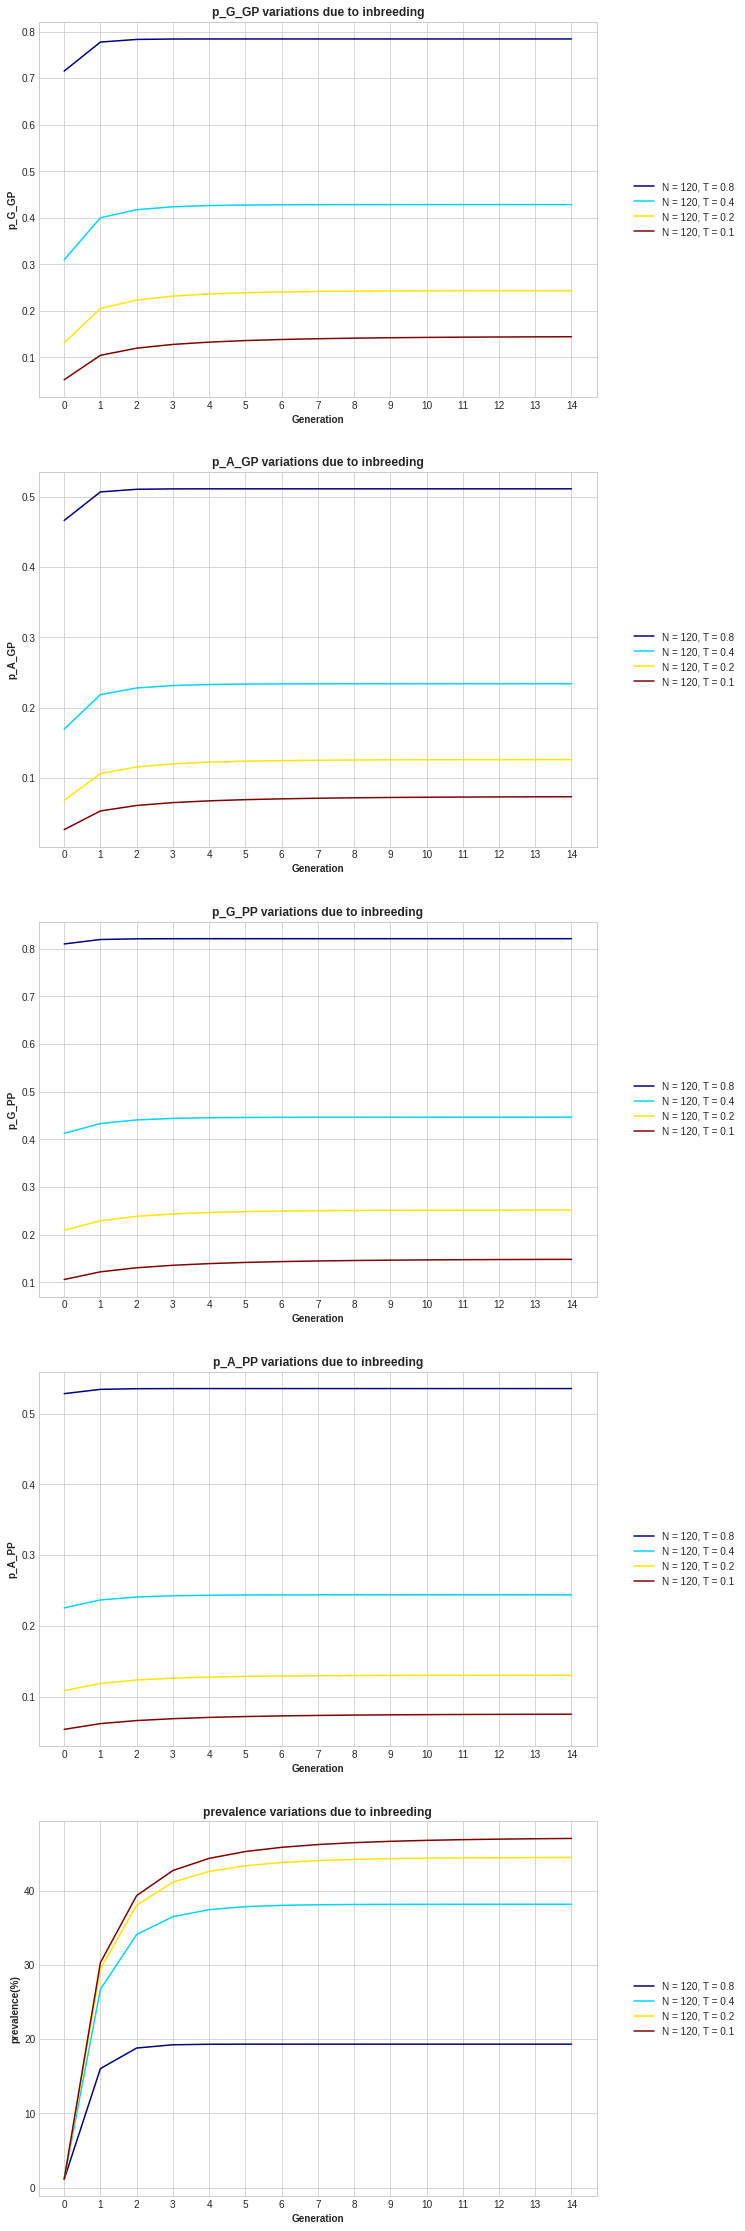
\includegraphics[scale=0.25]{Images/Gen_Analysis_Fix N.png}
    \caption{PP inbreeding analysis for fixed N}
    \label{fig:my_label}
\end{figure}
\begin{figure}[htbp]
    \centering
    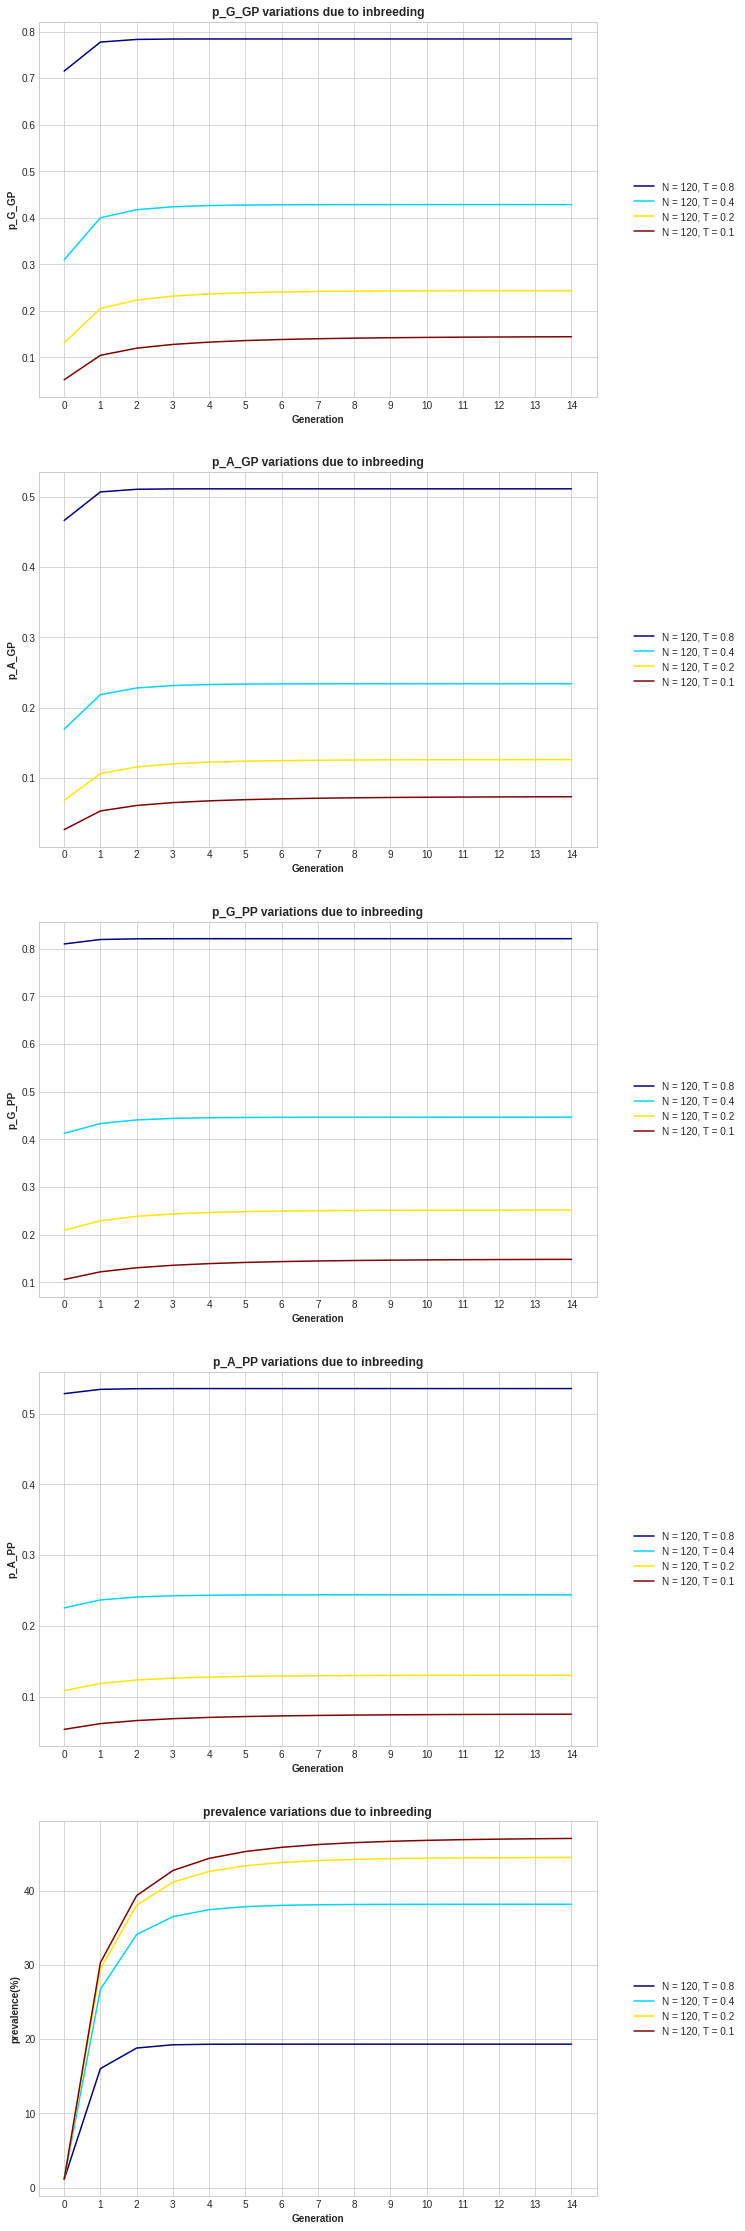
\includegraphics[scale=0.25]{Images/Gen_Analysis_Fix N.png}
    \caption{PP inbreeding analysis for fixed N}
    \label{fig:my_label}
\end{figure}
\begin{figure}[htbp]
    \centering
    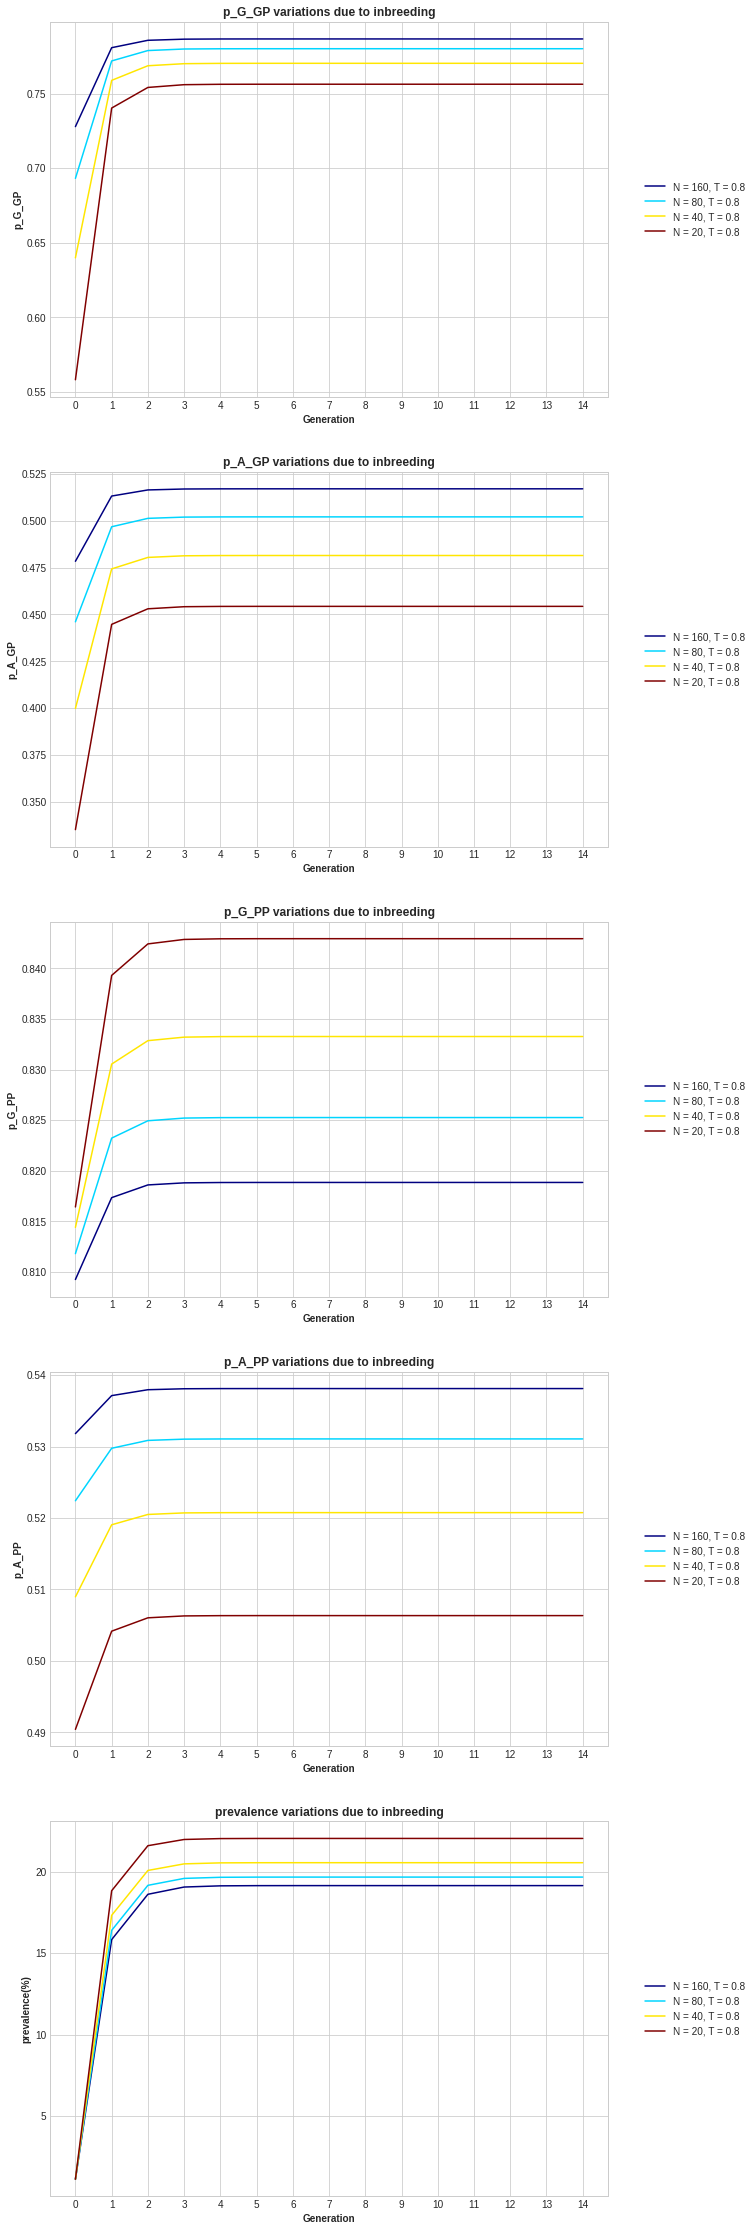
\includegraphics[scale=0.25]{Images/Gen_Analysis_Fix T.png}
    \caption{PP inbreeding analysis for fixed N}
    \label{fig:my_label}
\end{figure}
\begin{figure}[htbp]
    \centering
    \includegraphics[scale=0.25]{Images/Gen_Analysis_N&T_variation.png}
    \caption{PP inbreeding analysis for different N \& T}
    \label{fig:my_label}
\end{figure}

\bibliographystyle{IEEEtran}
\bibliography{ref.bib}

\end{document} 